% =============================================================================
%  Part VI -- The geometric limit: gravity from the response of the order
% =============================================================================

This part derives and tests the gravitational coupling of Causal Physics in the regime where
geometry is a reliable description of the order. It proceeds in five steps: what the coupling must
look like (Sec.~\ref{sec:tensor}), a substrate rule that realises it on causal sets
(Sec.~\ref{sec:rule}), why the rule follows from the action of the order (Sec.~\ref{sec:fromaction}),
a direct computation of that action to second order (Sec.~\ref{sec:bdaction}), and the static
propagator that turns the result into predictions (Sec.~\ref{sec:propagator}). The static section of
the field to first post-Newtonian order (Sec.~\ref{sec:static}) and the thermodynamic completion
beyond the linear order (Sec.~\ref{sec:jacobson}) close the part.

Conventions: signature $(-,+,+,+)$, $c=1$, $g=\eta+h$, $\bar h_{ab}=h_{ab}-\tfrac12\eta_{ab}h$. A static
weak field has $h_{00}=2U$, $h_{ij}=2\gamma U\delta_{ij}$, with $U>0$ the Newtonian potential and $u^a$
the four-velocity of the source.

% =============================================================================
\section{What the coupling must look like}\label{sec:tensor}
% =============================================================================

\subsection{The parameter \texorpdfstring{$\gamma$}{gamma} is a ratio of two couplings}

In the rest frame of a dust source, a static weak field with parameter $\gamma$ in $d_s$ spatial
dimensions has
\begin{equation}
  \bar h_{00}=U(1+\gamma d_s),\qquad \bar h_{ij}=U(1+2\gamma-\gamma d_s)\,\delta_{ij}.
\end{equation}
In 3+1 this is
\begin{equation}\label{eq:hbar-gamma}
  \bar h_{ab}=U\big[(1-\gamma)\,\eta_{ab}+2(1+\gamma)\,u_au_b\big].
\end{equation}
The field is a mixture of two couplings: to the trace of the energy--momentum tensor ($\eta_{ab}$) and
to the tensor itself ($u_au_b$).
\begin{itemize}
\item $\gamma=-1$: $\bar h_{ab}=2U\eta_{ab}$, pure trace coupling (spin 0, Nordstr\"om). Light is not
  deflected and does not gravitate, because the electromagnetic field has zero trace. This is the
  geometry of a fixed order (Sec.~\ref{sec:action}).
\item $\gamma=1$: $\bar h_{ab}=4U\,u_au_b$, pure coupling to $T_{ab}=\rho\,u_au_b$ with no trace part.
  This is linearised general relativity, $\Box\bar h_{ab}=-16\pi G\,T_{ab}$.
\item $\gamma=1/3$ (cones that only narrow) is a mixture of the two.
\end{itemize}

\subsection{The throughput principle is the tensor coupling}

The throughput principle $\rho_c\,c_{\rm eff}=\text{const}$ (Sec.~\ref{sec:response}) gives
$\gamma=2/(d_s-1)$. Pure tensor coupling of dust ($\bar h_{ij}=0$) gives $\gamma=1/(d_s-2)$. The two
coincide only for $d_s=3$. In three spatial dimensions, therefore, the throughput principle \emph{is}
the coupling of linearised general relativity: the deformation of the order lies only along the flow
($u_au_b$) and vanishes across it. Three consequences follow at once:
\begin{itemize}
\item light gravitates, and pressure gravitates as $\rho+3p$;
\item a moving source produces $g_{0i}$: inertial frames are dragged;
\item the field of many flows is a sum over flows, $\bar h_{ab}\propto\sum F\,u_au_b\,G_{\rm ret}$, whose
  transverse traceless part is a gravitational wave with the two polarisations $+$ and $\times$.
\end{itemize}

\subsection{A scalar field cannot be the whole law}

A single scalar clock field $\Pi$ in a fixed frame satisfies the static weak-field tests if the metric
is chosen with $\gamma=1$, but it cannot be the complete law of gravity. It has no $g_{0i}$, so it
cannot reproduce the frame dragging measured by Gravity Probe~B~\cite{Everitt2011}. Normalised to
Newton's law, a scalar field radiates quadrupole power
$P=\tfrac{G}{60}\big[(\mathrm{tr}\,\dddot I)^2+2\,\dddot I_{ij}\dddot I_{ij}\big]$, which for a circular
binary is exactly $1/6$ of the general relativistic value; binary pulsars agree with general relativity
to $10^{-3}$--$10^{-4}$~\cite{Kramer2021}. A scalar field is therefore the static section of the field in the rest frame
of its source, not the field itself (Sec.~\ref{sec:static}).

% =============================================================================
\section{The substrate rule and its test}\label{sec:rule}
% =============================================================================

\subsection{The rule}

The coupling of Sec.~\ref{sec:tensor} requires the order to know in which frame each flow is at rest.
The flows carry this information (Axiom~\ref{ax:momentum}). The substrate rule is:
\begin{enumerate}
\item \emph{own frame}: every flow narrows the causal cone in its own rest frame;
\item \emph{additivity}: flows that load the same relation share its capacity, and their cone deficits
  add;
\item \emph{throughput}: the density of events rises by $e^{\sigma_{\rm tot}}$, with $\sigma_i$ the
  rest-frame load of flow $i$ and $\sigma_{\rm tot}=\sum_i\sigma_i$.
\end{enumerate}
For a candidate relation with separation $d^a$ from an event loaded by flows with four-velocities
$u_i$, the relation is kept if and only if
\begin{equation}\label{eq:rule}
  d^0>0,\qquad -d_0^2+|\vec d|^2+\sum_i a_i\,(u_i\!\cdot d)^2\le0,\qquad
  a_i=\frac{\sigma_i}{\sigma_{\rm tot}}\big(1-e^{-2\sigma_{\rm tot}}\big).
\end{equation}
For flows at rest this is the single-flow throughput rule with cones narrowed to $e^{-\sigma_{\rm tot}}$.
The order is built from a flat sprinkling by keeping or discarding relations event by event; no metric
is sprinkled, and no field equation, Green function or trace reversal enters.

\subsection{The test: counter-streaming flows}

Two equally strong flows moving at $+v$ and $-v$ have zero momentum density but non-zero energy and
spatial stress. The candidate rules therefore predict different clock fields. With the rest-frame load
of each flow fixed, the amplitude of the clock field relative to $v=0$ is predicted to be:
\begin{center}
\begin{tabular}{lcc}
\toprule
rule & linear prediction & at $v=0.6$\\
\midrule
tensor rule \eqref{eq:rule} & $\Gamma_v^2(1+v^2)$ & $2.125$ (exact, non-linear: $2.361$)\\
energy density in the mean-flow frame & $\Gamma_v^2$ & $1.5625$\\
laboratory-frame density & $\Gamma_v$ & $1.25$\\
rest density (event count) & $1$ & $1$\\
\bottomrule
\end{tabular}
\end{center}
($\Gamma_v=1/\sqrt{1-v^2}$.) The amplitude is read in the near field, transverse to uniform flows, because
for a compact stationary system the stress integrates to zero (von Laue) and the $1/r$ tail cannot
distinguish the rules.

\paragraph{Result} (F7.4a, 3+1, 16 sprinklings per configuration, $\sim5.6\times10^4$ events,
\verdict{passed}). The blind instrument reads:
\begin{itemize}
\item amplitude ratio $R=A(0.6)/A(0)=2.401\pm0.053$ against $2.361$ for the tensor rule; the energy
  density reading ($1.5625$) is $16$ standard errors away. Pressure gravitates, not only energy;
\item cone anisotropy along/across the flows $K=1.221\pm0.012$ against $1.192$; every scalar rule of the
  mean-flow frame gives exactly $1$;
\item a single flow at $0.6c$ (reported): $R=2.538$ against $2.519$; the cone tilts, with a deficit
  against the flow $17.6$ times the deficit along it (prediction $12$, scalar rules $1$). The order drags
  its cones with the flow. The downstream deficit matches exactly ($-0.065$ against $-0.065$).
\end{itemize}
The flat control reads zero, and an isotropic order reads isotropic ($K=1.002\pm0.004$)
(Fig.~\ref{fig:counter}).

\begin{figure}[t]
  \centering
  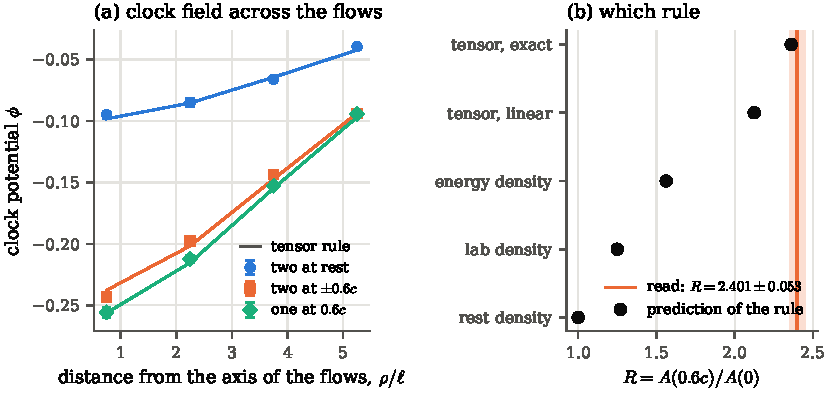
\includegraphics[width=\textwidth]{figures/fig_counter.pdf}
  \caption{Counter-streaming flows (F7.4a, 3+1, 16 sprinklings per configuration). (a) The clock potential read across the
flows (points, $\pm1$ standard error) against the tensor rule (lines) for two flows at rest, two flows at
$\pm0.6c$ and one flow at $0.6c$. (b) The amplitude ratio $R=A(0.6c)/A(0)$ read (orange line, band $\pm1$
standard error) against the prediction of each candidate rule.}\label{fig:counter}
\end{figure}

The test shows that a substrate with this rule couples to $T_{ab}$ as general relativity does at the
linear order, including frame dragging, with the tensor structure arising from the response of the order
alone. The rule itself is an input. The next section shows that it is not an independent one.

% =============================================================================
\section{The rule from the action of the order}\label{sec:fromaction}
% =============================================================================

\subsection{The matter side}

By Axiom~\ref{ax:action} the action of a flow is its proper time counted by the order. For $g=\eta+h$,
\begin{equation}
  \frac{\delta S_m}{\delta h_{ab}}=\tfrac12\,T^{ab}.
\end{equation}
Two parts of the substrate rule follow without any knowledge of the dynamics of the order:
\begin{itemize}
\item \emph{own frame}: the order sees a flow only through $u^au^b$, i.e.\ in the frame in which its
  proper time is measured;
\item \emph{additivity}: the action is a sum over flows, so at the linear order their contributions add.
\end{itemize}

\subsection{One number is left}

A linear, local and Lorentz-invariant response $h_{ab}=G*T$ has two channels, $T_{ab}$ and $\eta_{ab}T$.
For static dust this is the one-parameter family \eqref{eq:hbar-gamma}: the structure of the rule is
forced up to $\gamma$. The number $\gamma$ is fixed by the action of the order. For a general static
quadratic action coupled to dust,
\begin{equation}
  \mathcal L=c_{\Phi\Phi}|\nabla\Phi|^2+c_{\Phi\Psi}\nabla\Phi\cdot\nabla\Psi+c_{\Psi\Psi}|\nabla\Psi|^2
  -\kappa'\rho\,\Phi ,
\end{equation}
with $\dd s^2=-(1+2\Phi)\dd t^2+(1-2\Psi)\dd\vec x^2$, the variation with respect to $\Psi$ gives
\begin{equation}
  \gamma=\frac{\Psi}{\Phi}=-\frac{c_{\Phi\Psi}}{2\,c_{\Psi\Psi}},
\end{equation}
independently of $c_{\Phi\Phi}$. The Einstein--Hilbert action gives (computed symbolically for $d=2,3,4$)
\begin{equation}
  c_{\Phi\Phi}=0,\qquad c_{\Phi\Psi}=-2(d-1),\qquad c_{\Psi\Psi}=(d-1)(d-2)\quad\Rightarrow\quad
  \gamma=\frac{1}{d-2},
\end{equation}
which is $\gamma=1$ in 3+1. Two remarks:
\begin{itemize}
\item $c_{\Phi\Phi}=0$: clocks have no stiffness of their own; the time part of the field is fixed by
  the spatial part and the source.
\item The throughput principle is a consequence: dust has no stress and the order has the
  Einstein--Hilbert stiffness, so the trace-reversed spatial deformation vanishes.
\end{itemize}

\subsection{The chain}

With the Benincasa--Dowker action as the dynamics of the order (Axiom~\ref{ax:dynamics}):
\begin{equation*}
  \begin{gathered}
  \text{proper time counted by the order} \;+\; \text{BD action of the order}\\
  \Longrightarrow\;\text{the substrate rule at the linear order } (\gamma=1),
  \end{gathered}
\end{equation*}
provided the BD action has the Einstein--Hilbert stiffness. It is known that the expectation of the BD
action tends to the Einstein--Hilbert action, with a boundary term, in the continuum
limit~\cite{BenincasaDowker2010,MachetWang2020}.
The quantity that matters here, however, is the static quadratic form of the \emph{discrete} action at a
finite non-locality scale, including the contributions of long, nearly null intervals. The next section
computes it.

% =============================================================================
\section{The Benincasa--Dowker action to second order}\label{sec:bdaction}
% =============================================================================

\subsection{Sectors}

Write a static metric as $g=\Omega^2[-\dd t^2+n^2\dd\vec x^2]$ with $\omega=\ln\Omega$ and $\nu=\ln n$. The
conformal factor $\omega$ does not change the causal order, only the density of events; the optical
index $\nu$ changes the light cones. For plane waves $\omega=a\cos kz$, $\nu=b\cos kz$ the
Einstein--Hilbert action, averaged over a period, is (symbolic computation)
\begin{equation}\label{eq:EHquad}
  \Big\langle\sqrt{-g}\,R\Big\rangle=\frac{k^2}{2}\,\big(6a^2+8ab+2b^2\big)+O(a^3,b^3).
\end{equation}
Matter couples only to $\omega=\Phi$; in these variables $\gamma=-1+\cB/(2\cC)$ with $\cB=8$, $\cC=2$. We compute
here the conformal coefficient, $6$ in Einstein--Hilbert, which is an exact quadrature because the order
is unchanged.

\subsection{Method}

For $g=e^{2af}\eta$ with static $f$, the expected action per unit time and volume in the bulk of a region
of age $T$ (the past of every event cut at time $T$) is
\begin{equation}
  \Ex[S]=-2\big\langle\sqrt{-g}\;\Ex[B_\epsilon1](x)\big\rangle,
\end{equation}
with $\Ex[B_\epsilon1]$ from Eq.~\eqref{eq:Bexpect}. The proper volume of an interval is the flat
volume times the average of $e^{4af}$ over the interval. The second derivative with respect to $a$ at
$a=0$ is taken analytically under the integral: with $P=e^{4af}$, $\langle\cdot\rangle$ the average over the
interval, $g_1=w\,g_k'(w)$ and $g_2=w^2g_k''(w)$,
\begin{equation}
  \frac{\partial^2}{\partial a^2}\Big[P_xP_y\,g_k\big(w\langle P\rangle\big)\Big]_{a=0}
  =16\Big[(f_x+f_y)^2g_k+2(f_x+f_y)\langle f\rangle g_1+\langle f\rangle^2g_2+\langle f^2\rangle g_1\Big].
\end{equation}
The field is a static plane wave $f=\cos kz$, averaged over its phase in closed form, so that no wall
and no slowly converging tails enter. The averages of a plane wave over a causal interval are the
Fourier transform of the 3+1 causal diamond, which we use in closed form: in the rest frame of the
interval, with half-height $h$ and four-momentum $(\omega',q')$,
\begin{equation}
  F(\omega',q')=\frac{2}{V}\int_0^h\cos\big(\omega'(h-u)\big)\,
  \frac{4\pi\,(\sin q'u-q'u\cos q'u)}{q'^3}\,\dd u ,\qquad V=\frac{2\pi h^4}{3},
\end{equation}
evaluated stably for nearly null momenta. Lengths are in units of $\ell_k$ ($\epsilon\rho=1$); the
expectation depends on $\epsilon$ and $\rho$ only through their product. The result is reported as
\begin{equation}
  \hat K(k,T)=\frac{\partial_a^2\Ex[S]}{\text{Einstein--Hilbert value }6k^2}.
\end{equation}
The Einstein--Hilbert number enters only this normalisation.

\paragraph{Instruments} (all within tolerance): the closed-form transform agrees with an independent
quadrature of the diamond to $7\times10^{-8}$; the analytic second derivative agrees with finite
differences of the curved operator to $3\times10^{-4}$; a constant conformal factor gives zero response
to $5\times10^{-5}$ of the signal; doubling every quadrature parameter changes $\hat K$ by at most
$3\times10^{-5}$.

\subsection{Results}

For every wavenumber the response is linear in the age $T$ (residuals $\le10^{-3}$), so that
\begin{equation}\label{eq:Khat}
  \hat K(k,T)=K_{\rm loc}(k)-c_T\,k^3\,T .
\end{equation}

\begin{center}
\begin{tabular}{ccccccccccc}
\toprule
$k\ell_k$ & 0.025 & 0.035 & 0.05 & 0.07 & 0.1 & 0.14 & 0.2 & 0.3 & 0.5\\
\midrule
$K_{\rm loc}$ & 0.9904 & 0.9826 & 0.9680 & 0.9438 & 0.8994 & 0.8287 & 0.7056 & 0.4687 & $-0.015$\\
\bottomrule
\end{tabular}
\end{center}

\paragraph{The local part.} A fit $K_{\rm loc}=K_0-k^2[c_1\ln(1/k)+c_0]$ over $k\ell_k\le0.1$ gives
\begin{equation}
  K_0=1.00005,\qquad c_1=3.98,\qquad c_0=0.91,\qquad\text{rms }2.3\times10^{-5}.
\end{equation}
The conformal stiffness of the discrete BD action is therefore $6K_0=6.0003$: \emph{the Einstein--Hilbert
value emerges from the counting of intervals} (F6.8a, \verdict{passed}). The discreteness corrects it
non-analytically,
\begin{equation}
  1-K_{\rm loc}\simeq(k\ell_k)^2\big[4.0\ln(1/k\ell_k)+0.9\big],
\end{equation}
and the stiffness changes sign at $k\ell_k\simeq0.49$, a wavelength of $12.7\,\ell_k$. The momentum-space form
factor of the continuum non-local d'Alembertian is known in closed form~\cite{AslanbeigiSaravaniSorkin2014,
BelenchiaBenincasaLiberati2015}; a quantitative comparison of its infrared expansion with the non-analytic
correction found here is a planned independent check.

\paragraph{The age term.} The second term of Eq.~\eqref{eq:Khat} is not local: the static response
weakens in proportion to how long the field has existed. We predicted it before computing it. A long,
nearly null interval running perpendicular to $\vec k$ stays in phase with the field over its whole length.
Expanding its contribution in the proper time $\tau$ of the interval, the moment conditions of the BD kernel,
$\int u^{p}g_k(u)\,\dd u=0$ for $p=-\tfrac12,0,\tfrac12$, remove the orders $\tau^0$, $\tau^2$ and
$\tau^4$, but not $\tau^6$. Each unit length of history therefore adds a contribution of order $k^5$,
which is $k^3T$ relative to $k^2$. In the limit of long intervals the contribution depends only on the phase
$\phi=kL\cos\theta$ and on $k\tau$, and the coefficient is a two-dimensional integral of the diamond
transform,
\begin{equation}
  \frac{\dd J}{\dd T}=\frac{2\pi}{k}\int\dd\phi\int\tau\,\dd\tau\,
  \Big[2\cos\tfrac{\phi}{2}\,F\,g_1+\tfrac12F^2g_2\Big],
\end{equation}
which gives $c_T=0.1012$--$0.1022$ for $k\ell_k=0.05$--$0.2$. The full computation gives
$c_T=0.1035\pm0.0003$ for $k\ell_k\le0.2$ and $0.098$--$0.104$ over the whole range: agreement to $2\%$,
the rest being the finite age. In physical units the relative size of the age term is
\begin{equation}
  0.1\,(k\ell_k)^3\,\frac{T}{\ell_k}=0.1\,k^3\ell_k^2\,T .
\end{equation}
Figure~\ref{fig:conformal} shows the local part with its fit and the collapse of the age term.

\begin{figure}[t]
  \centering
  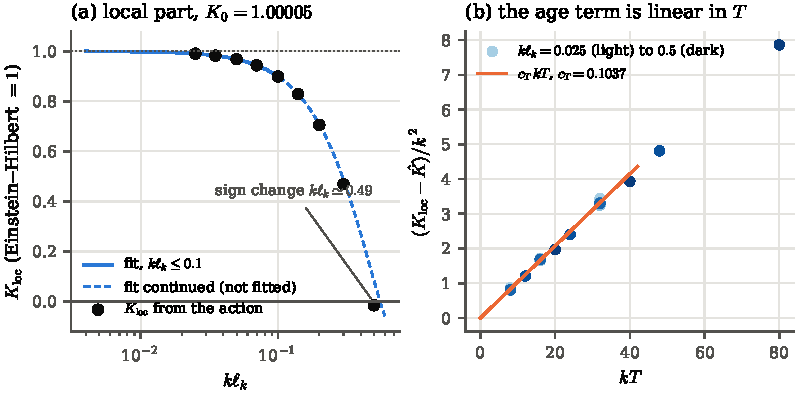
\includegraphics[width=\textwidth]{figures/fig_conformal.pdf}
  \caption{The conformal sector (F6.8a). (a) The local part $K_{\rm loc}$ of the stiffness in units of the
Einstein--Hilbert value (points), the fit $K_0-k^2[c_1\ln(1/k)+c_0]$ over $k\ell_k\le0.1$ (solid) and its
continuation (dashed), which the points beyond the fitted range follow to the sign change at
$k\ell_k\simeq0.49$. (b) The age term: $(K_{\rm loc}-\hat K)/k^2$ for every computed age and wavenumber (light to
dark: $k\ell_k=0.025$ to $0.5$) against $kT$, with the line $c_T\,kT$, $c_T$ the mean of the per-$k$ slopes over
$0.05\le k\ell_k\le0.2$. The two largest wavenumbers leave the line at large $kT$.}\label{fig:conformal}
\end{figure}

% =============================================================================
\section{Covariance and the static propagator}\label{sec:propagator}
% =============================================================================

\subsection{Form factors}

The expected BD action depends only on the geometry; it is exactly invariant under diffeomorphisms. If its
quadratic part around flat space is also covariant, it has the form
\begin{equation}
  S_2=\int\sqrt{-g}\,\Big[R+R\,F_0(\Box)\,R+C_{abcd}\,F_2(\Box)\,C^{abcd}\Big],
\end{equation}
the basis $\{R^2,C^2\}$ being complete at this order. For the plane waves of Eq.~\eqref{eq:EHquad},
$R^{(1)}=2k^2(3a+2b)\cos kz$ and $C^{(1)}\!\cdot C^{(1)}=\tfrac43\,b^2k^4\cos^2kz$: the Weyl tensor comes from
the optical index alone. Per $k^2/2$ the three coefficients become
\begin{equation}
  \cA=6+9\varphi_0,\qquad \cB=8+12\varphi_0,\qquad \cC=2+4\varphi_0+\varphi_2,\qquad
  \varphi_0=4k^2F_0,\quad \varphi_2=\tfrac43k^2F_2 .
\end{equation}

\subsection{The field of a point mass}

Matter couples to $\omega=\Phi$. Solving the quadratic form with a source gives the standard decomposition
into spin~2 and spin~0:
\begin{align}
  \frac{\Phi}{\Phi_{\rm GR}}&=\tfrac43S_2(k)-\tfrac13S_0(k), &
  \frac{\Psi}{\Psi_{\rm GR}}&=\tfrac23S_2(k)+\tfrac13S_0(k), &
  \gamma(k)&=\frac{2S_2+S_0}{4S_2-S_0},
\end{align}
with $S_0=1/(1+\tfrac32\varphi_0)$ and $S_2=1/(1-\tfrac32\varphi_2)$. Since $1+\tfrac32\varphi_0=\cA/6=\hat K$,
\emph{the computation of Sec.~\ref{sec:bdaction} determines the whole spin-0 channel}:
\begin{equation}
  S_0(k)=\frac{1}{\hat K(k,T)}=\frac{1}{K_{\rm loc}(k)-c_T\,k^3T}.
\end{equation}
The spin-0 propagator has a static pole where $\hat K=0$: at $k\ell_k\simeq0.49$ without the age term, and
with it at the length scale $(0.1\,\ell_k^2T)^{1/3}$.

These expressions assume that the quadratic action is covariant at every $k$. Section~\ref{sec:mixed}
tests this assumption directly.

\subsection{The mixed sector}\label{sec:mixed}

Covariance makes a sharp prediction without a free parameter: the mixed coefficient follows the
conformal one, $\cB/8=\cA/6=\hat K$ at every $k$. We computed $\cB$ directly (F6.8b2), for
$g=e^{2af}\big(-\dd t^2+e^{2bh}\dd\vec x^2\big)$ with $f=h=\cos kz$, phase-averaged.

\paragraph{Method.} The optical index changes the order. To first order in $b$, $y$ precedes $x$ if and
only if their time separation exceeds the optical length of the straight segment between them; by
Fermat's principle the change of the path is of second order. The past of $x$ is parametrised on the
unperturbed cone. The volume of an interval is the integral, over the spatial projection of the diamond
(a prolate spheroid, integrated in prolate spheroidal coordinates), of the time extent left by the
optical delays; the difference between the delay along the full segment and along the broken path is
formed pointwise, before averaging, so that thin intervals lose no digits. The age cut depends on $b$ and
contributes a boundary term, integrated on its own quadrature. The derivative $\partial_a\partial_b$ is
taken analytically, and the conformal $\hat K$ is computed on the same nodes and ages. The result is
reported as $\hat K_{ab}=\partial_a\partial_b\Ex[S]/(\text{Einstein--Hilbert value }4k^2)$.

\paragraph{Instruments} (all within tolerance): the derivatives of the interval volume agree with an
independent quadrature in spherical coordinates to $3.5\times10^{-5}$ and $5.8\times10^{-5}$; a uniform
optical index, a constant rescaling of space, changes no proper volume, to $9\times10^{-14}$; the
conformal $\hat K$ on this grid reproduces Sec.~\ref{sec:bdaction} to $2\times10^{-10}$; a constant
perturbation ($k=0$) gives zero response to $2.6\times10^{-4}$ in units of $\hat K$ at the smallest $k$,
for ages up to $T=320\,\ell_k$; doubling every quadrature parameter changes $\hat K_{ab}$ by at most
$3.2\times10^{-5}$.

\paragraph{Results.} For each $k$ the ages are $T=8,12,16$ times $1/k$ (at least $40\,\ell_k$), and
$\hat K_{ab}(k,T)=K_{{\rm loc},ab}(k)-c_{T,ab}\,k^3T$ is fitted as in Eq.~\eqref{eq:Khat}:
\begin{center}
\begin{tabular}{lccccc}
\toprule
$k\ell_k$ & 0.05 & 0.07 & 0.1 & 0.14 & 0.2\\
\midrule
$K_{{\rm loc},ab}$ (mixed) & 0.9683 & 0.9464 & 0.9045 & 0.8387 & 0.7261\\
$K_{\rm loc}$ (conformal, same ages) & 0.9681 & 0.9441 & 0.8999 & 0.8297 & 0.7076\\
$\Delta=K_{{\rm loc},ab}-K_{\rm loc}$ & 0.0002 & 0.0023 & 0.0046 & 0.0091 & 0.0184\\
$c_{T,ab}$ (mixed) & 0.155 & 0.197 & 0.195 & 0.195 & 0.195\\
$c_T$ (conformal) & 0.110 & 0.110 & 0.110 & 0.110 & 0.109\\
\bottomrule
\end{tabular}
\end{center}

\paragraph{The local part is covariant.} Over $k\ell_k\le0.1$ the largest difference is
$|\Delta|=4.6\times10^{-3}$, within the criterion fixed before the run ($\le10^{-2}$; F6.8b2,
\verdict{passed}). A fit $K_{{\rm loc},ab}=K_{0,ab}-k^2[c_1\ln(1/k)+c_0]$ over $k\ell_k\le0.14$ gives
$K_{0,ab}=0.9979$, i.e.\ a mixed stiffness
\begin{equation}
  \cB(k\to0)=8K_{0,ab}=7.983\qquad(\text{Einstein--Hilbert }8).
\end{equation}
Two of the three coefficients of the Einstein--Hilbert quadratic form, $6$ and $8$, therefore emerge from
the counting of intervals, and at leading order they stand in the covariant ratio.

\paragraph{Beyond the leading order the sectors differ.} For $k\ell_k=0.07$--$0.2$ the difference is a clean
analytic term,
\begin{equation}
  \Delta\simeq0.46\,(k\ell_k)^2\qquad(\Delta/k^2=0.475,\;0.462,\;0.462,\;0.461),
\end{equation}
and the age term of the mixed sector is $1.78$ times that of the conformal one ($c_{T,ab}\simeq0.195$ against
$0.110$). Neither is possible for a covariant quadratic action, local or not, which gives $\cB/8=\cA/6$ at every
$k$. The expected BD action is exactly diffeomorphism invariant, but a static field cut at age $T$ is not
a covariant configuration: the cut defines the rest frame of the field. Both differences may therefore
come from the cut rather than from the action; which of the two is open. The smallest wavenumber,
$k\ell_k=0.05$, has the longest ages of the grid and departs from both regularities
($\Delta=1.6\times10^{-4}$, $c_{T,ab}=0.155$); it is reported and not interpreted.

\paragraph{The field without assuming covariance.} Matter does not couple to $\nu$. Eliminating $\nu$
from the quadratic form $\cA\omega^2+\cB\omega\nu+\cC\nu^2$ gives $\nu=-\cB\omega/(2\cC)$, and therefore
\begin{equation}\label{eq:gammaABC}
  \gamma(k,T)=\frac{\cB}{2\cC}-1,\qquad
  \frac{\Phi}{\Phi_{\rm GR}}=\frac{-2}{\cA-\cB^2/(4\cC)} ,
\end{equation}
with $\cA$, $\cB$, $\cC$ the coefficients of the discrete action at wavenumber $k$ and age $T$ (Einstein--Hilbert:
$6$, $8$, $2$, giving $\gamma=1$ and $\Phi=\Phi_{\rm GR}$).

\subsection{The optical sector}\label{sec:optical}

The coefficient $\cC$ is the $\nu^2$ sector: the light cones to second order. For
$g=-\dd t^2+e^{2bh}\dd\vec x^2$, $h=\cos kz$, two things change at second order in $b$.

\paragraph{Bent rays.} The order is given by the optical distance, the minimum over paths of
$\int e^{bh}\,\dd l$ (Fermat). With $T=L+bT_1+b^2T_2$, $T_1=\int h\,\dd l$ along the straight segment and
\begin{equation}
  T_2=\tfrac12\!\int h^2\,\dd l-\tfrac12\!\iint\nabla_{\!\perp}h(l)\,G(l,l')\,\nabla_{\!\perp}h(l')\,\dd l\,\dd l',
\end{equation}
with $G(u,u')=u_<(d-u_>)/d$ the Green function of $-\dd^2/\dd l^2$ with fixed ends: bending lowers the optical
distance. Averaged over the phase of the wave, for a segment of length $d$ with phase advance $p=\vec k\cdot\vec e\,d$,
\begin{equation}
  \langle T_2\rangle=\frac d4-\frac14\big(k^2d^2-p^2\big)\,d\,J(p),\qquad J(x)=\frac{x^2+2\cos x-2}{x^4}.
\end{equation}

\paragraph{Interval volumes.} The volume $V=\int\dd^3z\,P(z)\,[\Delta t-T(y,z)-T(z,x)]_+$ acquires, besides the
second derivatives of its integrand, a surface term $\int\delta(\ell_0)\,\ell'^2$ on the spatial projection of
the diamond. Differences of nearly equal path lengths are formed analytically so that long, thin intervals
lose no digits. The age cut depends on $b$ and contributes boundary terms, among them an edge term from pairs
that leave the past; it cancels a part of order $T^4$ of the other boundary terms exactly and is combined with
it analytically.

\paragraph{Instruments} (all within tolerance): the closed form of $\langle T_2\rangle$ agrees with rays found by
direct numerical minimisation of the optical length to $8\times10^{-5}$; the second derivative of the volume of
a test interval agrees with an independent computation (numerical roots of $\ell(b)=0$, numerical Green
function, finite differences in $b$) to $7\times10^{-4}$; a constant index gives zero to $4\times10^{-15}$; a
constant perturbation of the whole past gives zero to $3\times10^{-4}$ in units of $\hat K_{bb}$; doubling every
quadrature parameter changes $\hat K_{bb}$ by at most $7\times10^{-4}$.

\paragraph{The age dependence is not linear.} The first computation read the optical sector as the other two,
by a fit linear in the age at each $k$, and failed by its own criterion (F6.8c, \verdict{failed}): $\hat K_{bb}$
falls faster than linearly with $T$, and the linear extrapolation carries no information. In units
$\ell_k=1$ the age-dependent part of every sector scales as $k^2F(kT)$ (the conformal and mixed data obey this to
$10^{-4}$), so at fixed $n=kT$
\begin{equation}
  \hat K(k,n/k)=K_0-k^2\big[c_1\ln(1/k)+c_0(n)\big],
\end{equation}
and the intercept $K_0$ is the long-wavelength stiffness whatever $F$ is. The revision F6.8c2 applies this
reading to fresh wavenumbers ($k\ell_k=0.06$, $0.085$, $0.12$, $0.17$; $n=6$, $8$, $10$; ages up to $167\,\ell_k$);
the same reading of the conformal sector of the same rows returns $K_0=0.99976$ against $1.00005$.

\begin{center}
\begin{tabular}{lccc}
\toprule
$n=kT$ & $6$ & $8$ & $10$\\
\midrule
$K_{0,bb}$ (optical) & $0.99971$ & $1.00118$ & $0.97108$\\
$K_0$ (conformal, same rows) & $0.99976$ & $0.99976$ & $0.99977$\\
\bottomrule
\end{tabular}
\end{center}

\paragraph{Result.} At the pre-registered $n=8$, $K_{0,bb}=1.00118$ (F6.8c2, \verdict{passed}), so
\begin{equation}
  \cC(k\to0)=2K_{0,bb}=2.002\qquad(\text{Einstein--Hilbert }2).
\end{equation}
All three coefficients of the Einstein--Hilbert static form, $6$, $8$ and $2$, emerge from the counting of
intervals, and with them
\begin{equation}
  \gamma(k\to0)=\frac{2K_{0,ab}}{K_{0,bb}}-1=0.997\ \text{to}\ 1.000 ,
\end{equation}
the range spanning the readings at $n=6$ and $8$ (with $K_{0,ab}=0.99988$, the mixed sector read in the same way). $\gamma=1$ follows from the action of the order with nothing
from general relativity put in (Fig.~\ref{fig:sectors}). At $n=10$ the reading is pulled by its oldest row ($k\ell_k=0.06$,
$T=167\,\ell_k$), where doubling the quadrature also changes most; in the computation that failed, rows with
$T\gtrsim170\,\ell_k$ broke the scaling, which points to a numerical limit at large ages rather than to physics.
This is not settled.

\begin{figure}[t]
  \centering
  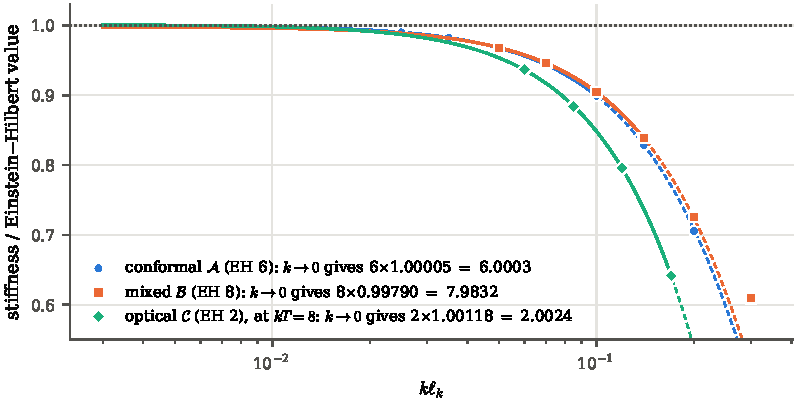
\includegraphics[width=\textwidth]{figures/fig_sectors.pdf}
  \caption{The three sectors of the static quadratic form approach the Einstein--Hilbert values as $k\to0$ (F6.8a,
F6.8b2, F6.8c2). Conformal $\cA$ and mixed $\cB$: the local part of the stiffness; optical $\cC$: $\hat K_{bb}$
at the pre-registered $n=kT=8$, which contains the age part $k^2c_0(8)$. Lines: the fits
$K_0-k^2[c_1\ln(1/k)+c_0]$ over the fitted range (solid) and continued (dashed). The intercepts give $6.0003$,
$7.983$ and $2.002$ against $6$, $8$ and $2$.}\label{fig:sectors}
\end{figure}

\paragraph{The age term of the optical sector.} Within the computed range the optical sector weakens with age
faster than linearly: at $k\ell_k=0.12$ the age part $k^2F_{bb}(n)$ grows between $n=6$, $8$, $10$, $16$ and $24$ by
increments that increase with $n$, whereas the conformal and mixed sectors become linear from $n\simeq8$
($c_T\simeq0.110$ and $0.195$). A local fit of the form $sn+qn^2$ is not stable: its coefficients depend on the
range of $n$, and they do so for the conformal sector as well below $n\simeq8$, where its linear asymptotics has
not yet set in. The data therefore do not fix the form of the optical age term; its behaviour as $kT\to\infty$,
the regime of any physical field, is open, and the predictions of the age term depend on it
(Part~\ref{part:predictions}; Fig.~\ref{fig:optical}).

\begin{figure}[t]
  \centering
  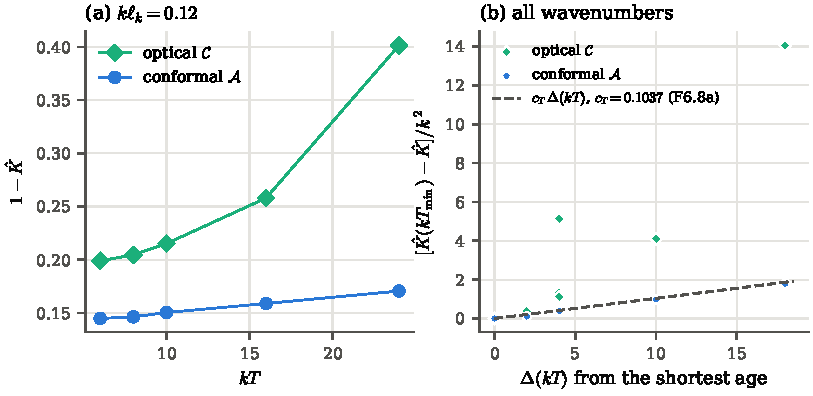
\includegraphics[width=\textwidth]{figures/fig_optical.pdf}
  \caption{The age dependence of the optical sector (F6.8c2). (a) $1-\hat K$ at $k\ell_k=0.12$ for $n=kT=6$, $8$, $10$,
$16$ and $24$, optical and conformal sectors of the same rows. (b) The decrease of $\hat K$ from the shortest
computed age, divided by $k^2$, for all wavenumbers: the conformal points follow the linear age term
$c_T\,\Delta(kT)$ of F6.8a, the optical points lie above it and grow faster than linearly.}\label{fig:optical}
\end{figure}

\subsection{What remains}

The asymptotic form of the age term in the optical sector, analytically as for the conformal one; the origin of
the differences between the sectors beyond the leading order (the age cut or the action); and the field of a
point mass by Fourier inversion of Eq.~\eqref{eq:gammaABC}. These are the next computations
(Part~\ref{part:predictions}).

% =============================================================================
\section{The static section to first post-Newtonian order}\label{sec:static}
% =============================================================================

In the rest frame of a static source the field reduces to the clock rate $\Pi$ with the metric fixed by
the throughput principle,
\begin{equation}
  \dd s^2=-\Pi^2\dd t^2+\Pi^{-2}\dd\vec x^2=-e^{2L}\dd t^2+e^{-2L}\dd\vec x^2,\qquad L=\ln\Pi .
\end{equation}
The static field equation is the BD operator of the order acting on the logarithm of the clock rate,
\begin{equation}\label{eq:static}
  B_g\ln\Pi=\kappa\rho_s
  \;\longrightarrow\;
  e^{2L}\big[(1-L)\Delta L+L|\nabla L|^2\big]=\kappa\rho_s
\end{equation}
in the continuum limit $B_g\to\Box_g-\tfrac12R$. In the weak field $\Delta L=\kappa\rho_s$, so $L=-U$ with
$\kappa\rho_s\leftrightarrow4\pi G\rho$. The choice of the logarithm is fixed by observation: for
$B_gf(\Pi)=\kappa\rho_s$ the post-Newtonian parameter is $\beta=(1-f''(1))/2$, and only $f''(1)=-1$, i.e.\ the
logarithm in the family $(\Pi^k-1)/k$, gives $\beta=1$, required by the perihelion advance. The logarithm
also turns the multiplicative composition of clock ratios into an additive potential.

This equation is the static section of the field to first post-Newtonian order ($\gamma=\beta=1$). It is not
the complete law: beyond this order the field is the full tensor field of Sec.~\ref{sec:tensor}, completed
by general relativity (Sec.~\ref{sec:jacobson}).

% =============================================================================
\section{Thermodynamic completion}\label{sec:jacobson}
% =============================================================================

Beyond the linear order the coupling to the total conserved energy--momentum, including that of the field
itself, determines the theory uniquely: it is general relativity~\cite{Deser1970,FeynmanGravitation,Lovelock1971}.
Causal Physics adopts this completion and aims to \emph{derive} it from the order, following
Jacobson~\cite{Jacobson1995}: if every local causal horizon carries an entropy proportional to its area with a
universal constant, the Clausius relation $\delta Q=T_{\rm U}\,\delta S$ for every local Rindler horizon, with the Unruh
temperature $T_{\rm U}$, implies Einstein's equations as an equation of state,
\begin{equation}
  R_{ab}-\tfrac12Rg_{ab}+\Lambda g_{ab}=8\pi G\,T_{ab},\qquad G=\frac{1}{4\hbar\eta}.
\end{equation}

What the order supplies:
\begin{itemize}
\item \emph{Entropy proportional to area.} The number of horizon molecules measures the proper area of a
  horizon (K.14, Sec.~\ref{sec:reading}).
\item \emph{Matter with energy--momentum.} Flows carry four-momentum and have a measured $T_{ab}$
  (Axiom~\ref{ax:momentum}, K.15).
\item \emph{The linear Clausius condition.} For local Rindler horizons, the Clausius relation is equivalent to
  $R_{ab}k^ak^b=8\pi G\,T_{ab}k^ak^b$ for every null direction $k$. A clock field written in a fixed frame
  violates it for moving sources; the same field written in the rest frame of each source satisfies it exactly,
  which is linearised general relativity. The condition thus requires the field to carry the four-velocity of
  its sources, which is the substrate rule of Sec.~\ref{sec:rule}.
\end{itemize}
What remains open is the Clausius relation beyond the linear order, with a dynamics of the order that responds
to matter, and the Unruh temperature~\cite{Unruh1976}, which is an input from quantum field theory. The cosmological constant
appears as an integration constant, consistently with its origin as a fluctuation of the number of events
(Sec.~\ref{sec:onto-vacuum}).
